% Copyright 2007 by Till Tantau
%
% This file may be distributed and/or modified
%
% 1. under the LaTeX Project Public License and/or
% 2. under the GNU Public License.
%
% See the file doc/licenses/LICENSE for more details.


\lecture[24]{Using linear regression}{lecture-text}

\subtitle{confidence intervals, outliers, and leverage}

\date{28 April 2015}

% pp. 505-527


\begin{document}

\begin{frame}
  \maketitle
\end{frame}


\begin{frame}\frametitle<presentation>{Outline}
  \tableofcontents
\end{frame}


\section{The linear model}

%%%%%%
\begin{frame}{Conditional means, SDs}

  \begin{block}{Notation}
    \begin{align*}
      \mu_{Y|X} &= \; \text{mean value of $Y$ given $X$} \\
      \sigma_{Y|X} &= \; \text{SD of $Y$ given $X$} \\
    \end{align*}
  \end{block}


    \vspace{2em}

    \structure{Example:}
    Drug dose ($X$) and blood pressure ($Y$) in patients. \\
    $\mu_{Y|X}$ is the mean blood pressure among patients with dose $X$; \\
    $\sigma_{Y|X}$ is the SD.

\end{frame}

%%%%%%
\begin{frame}{The linear model}

  \structure{In words,} the values of $Y$ are normally distributed with mean
  a linear function of $X$ and a standard deviation that does not depend on $X$:
  \begin{align*}
    \mu_{Y|X} &= \beta_0 + \beta_1 X \\
    \sigma_{Y|X} &= \sigma_\epsilon
  \end{align*}
  or, equivalently,
  \begin{align*}
    Y = \beta_0 + \beta_1 X + \epsilon \\
    \epsilon \; \text{independent, with SD $\sigma_\epsilon$} .
  \end{align*}

\end{frame}


%%%%%%
\begin{frame}{Why linear?}

  \begin{enumerate}
      
    \item It is arguably the simplest possible relationship between $X$ and $Y$,
      requiring only two parameters ($b_0$ and $b_1$)

    \item Most things look linear at the right level of approximation.

    \item The mathematics works out nicely.

    \item Nonlinear relationships can often be transformed to linear relationships.

  \end{enumerate}

\end{frame}


\section{Estimates from data}


%%%%%%
\begin{frame}{Conditions}

  We clearly need some sort of \structure{independence} in the $(X,Y)$ data to make good estimates.

    \vspace{2em}

    \begin{block}{Random Subsampling Model}
      Each observed pair $(x_i,y_i)$ can be regarded as having $y_i$ sampled
      at random from the \alert{conditional} population of $Y$ values having the $X$ value $x_i$,
      and independent of the other samples.
    \end{block}

    \vspace{2em}

    \structure{Examples:}
    \begin{itemize}
      \item Heights ($X$), weights ($Y$) of a random sample from a populations.
      \item Clotting rate ($Y$) after a dose ($X$) of warfarin was administered,
        with dose assigned randomly.
    \end{itemize}

\end{frame}

%%%%%%
\begin{frame}{Parameter estimates}

  \begin{align*}
    Y = \beta_0 + \beta_1 X + \epsilon \\
    \epsilon \; \text{independent, with SD $\sigma_\epsilon$} .
  \end{align*}
  \vspace{2em}

  If the random subsampling model holds, then
  \begin{enumerate}
    \item[$b_0$] is an estimate of $\beta_0$ (the intercept)
    \item[$b_1$] is an estimate of $\beta_1$ (the slope)
    \item[$s_e$] is an estimate of $\sigma_\epsilon$ (the SD of the noise)
  \end{enumerate}

\end{frame}


%%%%%%
\begin{frame}{Example: Galton 1885}

  Son's height ($Y$) and ``midparent'' height, in inches \\
  (average of: father's and 1.08 $\times$ mother's heights)
  \begin{center}
    \includegraphics<1>{galton.pdf}
  \begin{align*}
    \hat \mu_X &= 68.31 & s_X &= 1.79 & s_e &= 2.24 
    \hat \mu_Y &= 68.09 & s_Y &= 2.52 & r &= 0.459 \\
  \end{align*}
  \begin{align*} 
    \text{(son's height)} &= 68.09 + 0.459 \times \frac{2.52}{1.79} \times \left( \text{(midparent height)} - 68.31 \right) + \epsilon  \\
    &= 24 + 0.64 \times \text{(midparent height)}  + \epsilon
  \end{align*}

  \end{center}

\end{frame}


%%%%%%
\begin{frame}{}
  \begin{center}
    \begin{align*} 
      Y &= \beta_0 + \beta_1 X + \epsilon \\
      \text{(son's height)} &= 24 + 0.64 \times \text{(midparent height)}  + \epsilon\\
      s_e &= 2.24
    \end{align*}
  \end{center}
  \begin{enumerate}
    \item How tall is the average offspring of parents with midparent height 70"?
      \pause
      \[  24 + 0.64 \times 70  = 68.8 \]
      \pause
    \item \ldots for midparent height 66"?
      \pause
      \[  24 + 0.64 \times 66  = 66.2 \]
      \pause
    \item Is a child 62" tall with midparent height 66" suprising?
      \pause
      \[  z = \frac{62 - (24+0.64\times 66)}{2.24} = 1.89 \]
      \pause
    \item \ldots how about a child 73" tall?
      \pause
      \[  z = \frac{73 - (24+0.64\times 66)}{2.24} = 3.02 \]
  \end{enumerate}

\end{frame}


\section{Inference on the slope}

%%%%%%
\begin{frame}{The standard error of the slope}


  \begin{block}{Standard Error for $b_1$}
      \[
          \SE_{b_1} = \frac{ s_e }{ s_x \sqrt{n-1} }
      \]
  \end{block}

    \vspace{2em}
    
    \only<1>{
        \begin{center}
        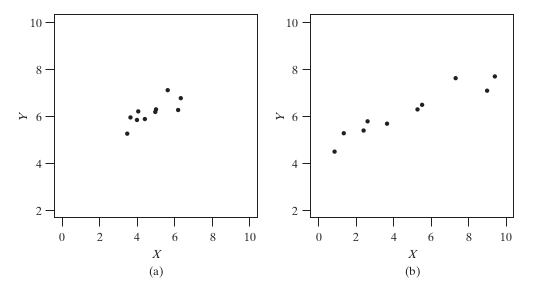
\includegraphics[width=3in]{fig-12-5-1.png}
        \end{center}
    }
    \pause

    Intuitively,
    we will be more certain about the relationship with
    \begin{itemize}
        \item less noise in the relationship ($s_e$)
        \item larger sample size ($n$)
        \item a wider spread of $x$ values ($s_x$)
    \end{itemize}

    \vspace{2em}

    A \alert{95\% confidence interval} for the slope is:
    \[
        b_1 \pm t_{n-2,0.025} \SE_{b_1} .
    \]

\end{frame}


%%%%%%
\begin{frame}{Hypothesis testing}

    As usual with $\SE_{b_1}$: \\
    Under a null hypothesis of no relationship,
    \[
        H_0: \; \beta_1 = 0 ,
    \]
    the independent subsampling model, \\
    and normally distributed deviations with equal variance, \\
    the test statistic 
    \[
        t_s = \frac{b_1 - 0}{\SE_{b_1}}
    \]
    is $t$-distributed with $n-2$ degrees of freedom.

    \vspace{2em}

    \structure{Note:} this is the \alert{same} as our previous test of no correlation.

\end{frame}

%%%%%%%

\begin{frame}{Conditions}

  Statistical \alert{inference} using linear regression
  requires:
  \begin{enumerate}
    \item Independent pairs $(X,Y$) from either:
      \begin{itemize}
        \item random subsampling (of $Y$ given $X$), \structure{or}
        \item bivariate random sampling (of pairs $(X,Y)$)
      \end{itemize}
    \item Under the \structure{linear model},
      \begin{align*}
        \mu_{Y \given X} &= \beta_0 + \beta_1 X \\
        \sigma_{Y \given X} &\; \text{does not depend on $X$}.
      \end{align*}
    \item To use the $t$ distribution for $b_1$, \\
      the conditional population distribution of $Y$ given $X$ \\
      must be normally distributed.
  \end{enumerate}

\end{frame}

\begin{frame}{Example: growth of Loblolly pines}

  Heights and ages of 84 Loblolly pines, \alert{$r=0.99$}:
  \begin{center}
    \includegraphics<1>{loblolly-age-height}
  \end{center}

    \begin{center}
        \begin{tabular}{r|rr}
          & mean & SD \\
          \hline
          age & 13.0 & 7.9 \\
          height & 32.4 & 20.6 \\
        \end{tabular}
    \end{center}

    \pause
  \begin{align*}
    \text{(height)} &= 32.4 + 0.99 \times \frac{20.6}{7.9} (\text{(age)}-13) + \epsilon \\
        &= -1.3 + 2.6 \times \text{(age)} \\
        s_e &= 2.95 \\
  \end{align*}
  \pause
  \begin{align*}
        \SE_{b_1} &= \frac{2.95}{7.9\sqrt{84-1}} = 0.041 \\
        t_s &= \frac{2.6 - 0}{0.041} = 63.3
  \end{align*}

\end{frame}


%%%% %%%%%%% %%%%%%%
\section{Interpretation}


%%%%%%
\begin{frame}{Residuals}

  \ldots are what's left over, $e_i$:
  \begin{align*}
    \hat y_i &= b_0 + b_1 x_i \\
    e_i &= y_i - \hat y_i
  \end{align*}

  \begin{center}
    \includegraphics<1>{loblolly-age-height}
    \includegraphics<2>{loblolly-resids}
  \end{center}

  \vspace{1em}
  \alert{What does this mean?}

\end{frame}


%%%%%%
\begin{frame}{Nonlinearity}

    \begin{center}
    \includegraphics<1>{nonlinear1.pdf}
    \includegraphics<2>{nonlinear2.pdf}
    \end{center}

    If the true relationship isn't linear, \\
    then linear regression might not be the right tool.
    \pause

    \alert{But it might be a good first pass.}


\end{frame}




\section{Diagnostic plots}


%%%%%%
\begin{frame}{Residuals versus predicted}
    Checks for nonlinearity; \uncover<3->{heteroskedasticity (different variances)}
    \begin{center}
        \includegraphics<1>{nonlinear2-resids.pdf}
        \includegraphics<2>[width=\textwidth]{usc-temps-fit-resid.pdf}
        \includegraphics<3>{hetersked-resids.pdf}
    \end{center}

    \structure{The hope} is to see \alert{no structure} in the residual plot.

\end{frame}


% 
% %%%%%%
% \begin{frame}{What can go wrong?}
% 
%     \begin{center}
%         \includegraphics[width=\textwidth]<1>{many-regressions-1.pdf}
%         \includegraphics[width=\textwidth]<2>{many-regressions-2.pdf}
%         \includegraphics[width=\textwidth]<3>{many-regressions-3.pdf}
%     \end{center}
% 
% \end{frame}



\begin{frame}{Common errors: nonindependence}


  \alert{ Observations are dependent: } \\

  20 measurements of serum cholesterol ($X$) and glucose ($Y$) \ldots \\
  10 from each patient.
  \vspace{2em}

      \structure{Example:} 
      \begin{center}
        \includegraphics<1>[width=\textwidth]{nonindep-0}
        \includegraphics<2>[width=\textwidth]{nonindep}
      \end{center}

\end{frame}


\begin{frame}{Common errors: misinterpretation}
    
  $r$ estimates the \alert{population correlation} $\rho$ \\
  \structure{only}
  under the bivariate random sampling model.

  \vspace{2em}


      \structure{Example:} 
      \begin{center}
        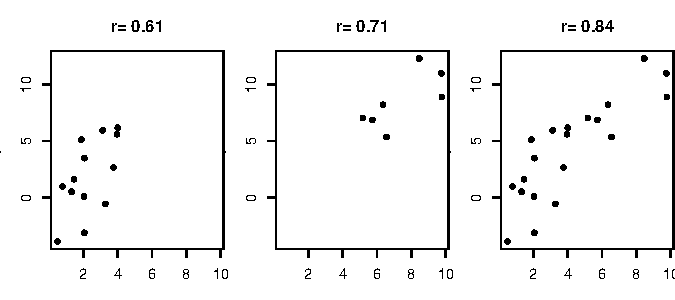
\includegraphics[width=\textwidth]{r-interp}
      \end{center}


\end{frame}

\begin{frame}{Example: Loblolly}
  Heights and ages of 84 Loblolly pines, \alert{$r=0.99$}:
  \begin{center}
    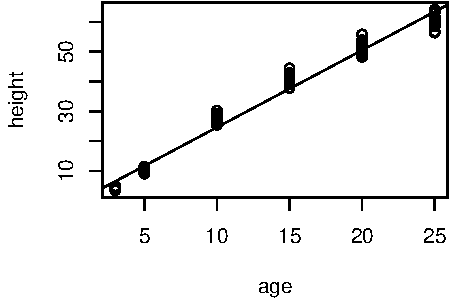
\includegraphics{loblolly-age-height}
  \end{center}

  \vspace{1em}
  
  What's wrong with this:

  ``Tree age explains 98\% of the variance of Loblolly pine height in the forest.''

\end{frame}



%%%%%%
\begin{frame}{Outliers}

    An \alert{outlier} is a data point unusually far from the rest (in some sense; usually in the sense of having \alert{large residuals}).
    \begin{center}
        \includegraphics<1>[width=3in]{fig-12-6-3.png}
        \includegraphics<2>[width=2in]{fig-12-6-3.png}
    \end{center}
    \pause

    These usually indicate deviations from the model;\\
    and may have a large effect on the results.


    \vspace{2em}

    \structure{What to do:} investigate, use robust statistics.

\end{frame}


%%%%%%
\begin{frame}{Leverage points}

    A \alert{leverage point} is one that \emph{could} have a large effect on the regression.
    (i.e.\ moving it changes the slope of the regression line a lot)
    \begin{center}
        \includegraphics<1>[width=3in]{fig-12-6-3.png}
        \includegraphics<2>[width=2in]{fig-12-6-3.png}
    \end{center}
    \pause

    \vspace{1em}

    These are \structure{far from the center of mass}.


    \vspace{1em}

    \structure{What to do:} investigate.

\end{frame}



%%%%%%
\begin{frame}{Influential points}

    An \alert{influential point} is one that actually \alert{is} affecting the regression line a lot -- if it was removed, the slope would change dramatically.
    \begin{center}
        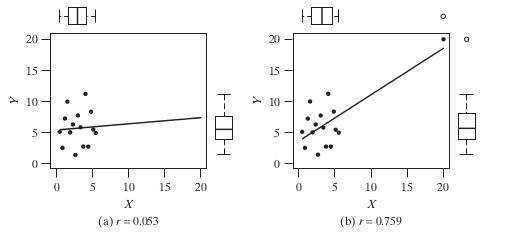
\includegraphics[width=3in]{fig-12-6-4.png}
    \end{center}

    \vspace{2em}

    \structure{What to do:} investigate.

\end{frame}


\section<article>{Summary}
\section<presentation>*{Summary}

\begin{frame}{Summary}
  \begin{enumerate}
      \item Linear regression fits a model where the mean of $Y$ is a linear function of $X$
      \item and the variances do not depend on $X$.
      \item Under the ``random subsampling model'',
      \item $b_0$ and $b_1$ are good estimates of the terms in the linear relationship
      \item and $s_e$ is a good estimate of the residual SD.
      \item Testing for correlation is equivalent to testing for $b_1=0$,
      \item which we can do with a $t$ test and $\SE_{b_1}$.
      \item Look at the data to check if the conditions are met.
  \end{enumerate}
\end{frame}

% homework
\begin{frame}{Homework}
  \begin{center}

      Two 8.5"$\times$11" pages, two-sided, of handwritten notes.

    \vspace{2em}

    Bring a calculator (besides your phone).

  \end{center}
\end{frame}


\end{document}





